%%%%%%%%%%%%%%%%%%%%%%%%%%%%%%%%%%%%%%%%%
% Jacobs Landscape Poster
% LaTeX Template
% Version 1.0 (29/03/13)
%
% Created by:
% Computational Physics and Biophysics Group, Jacobs University
% https://teamwork.jacobs-university.de:8443/confluence/display/CoPandBiG/LaTeX+Poster
% 
% Further modified by:
% Nathaniel Johnston (nathaniel@njohnston.ca)
%
% This template has been downloaded from:
% http://www.LaTeXTemplates.com
%
% License:
% CC BY-NC-SA 3.0 (http://creativecommons.org/licenses/by-nc-sa/3.0/)
%
%%%%%%%%%%%%%%%%%%%%%%%%%%%%%%%%%%%%%%%%%

%----------------------------------------------------------------------------------------
%	PACKAGES AND OTHER DOCUMENT CONFIGURATIONS
%----------------------------------------------------------------------------------------

\documentclass[final]{beamer}
\usepackage[utf8]{inputenc}

\usepackage[scale=1.24]{beamerposter} % Use the beamerposter package for laying out the poster

\usetheme{confposter} % Use the confposter theme supplied with this template

\setbeamercolor{block title}{fg=ngreen,bg=white} % Colors of the block titles
\setbeamercolor{block body}{fg=black,bg=white} % Colors of the body of blocks
\setbeamercolor{block alerted title}{fg=white,bg=dblue!70} % Colors of the highlighted block titles
\setbeamercolor{block alerted body}{fg=black,bg=dblue!10} % Colors of the body of highlighted blocks
% Many more colors are available for use in beamerthemeconfposter.sty

%-----------------------------------------------------------
% Define the column widths and overall poster size
% To set effective sepwid, onecolwid and twocolwid values, first choose how many columns you want and how much separation you want between columns
% In this template, the separation width chosen is 0.024 of the paper width and a 4-column layout
% onecolwid should therefore be (1-(# of columns+1)*sepwid)/# of columns e.g. (1-(4+1)*0.024)/4 = 0.22
% Set twocolwid to be (2*onecolwid)+sepwid = 0.464
% Set threecolwid to be (3*onecolwid)+2*sepwid = 0.708

\newlength{\sepwid}
\newlength{\onecolwid}
\newlength{\twocolwid}
\newlength{\threecolwid}
\setlength{\paperwidth}{48in} % A0 width: 46.8in
\setlength{\paperheight}{36in} % A0 height: 33.1in
\setlength{\sepwid}{0.024\paperwidth} % Separation width (white space) between columns
\setlength{\onecolwid}{0.22\paperwidth} % Width of one column
\setlength{\twocolwid}{0.464\paperwidth} % Width of two columns
\setlength{\threecolwid}{0.708\paperwidth} % Width of three columns
\setlength{\topmargin}{-0.5in} % Reduce the top margin size
%-----------------------------------------------------------

\usepackage{graphicx}  % Required for including images

\usepackage{booktabs} % Top and bottom rules for tables

%----------------------------------------------------------------------------------------
%	TITLE SECTION 
%----------------------------------------------------------------------------------------

\title{Computation offloading with ICN} % Poster title

\author{Michał Król, Adrian-Cristian Nicolaescu, Sergi Reñé, Onur Ascigil, Ioannis Psaras, David Oran, Dirk Kutscher} % Author(s)

\institute{University College London, Network Systems Research \& Design, Huawei} % Institution(s)

%----------------------------------------------------------------------------------------

\begin{document}

\addtobeamertemplate{block end}{}{\vspace*{2ex}} % White space under blocks
\addtobeamertemplate{block alerted end}{}{\vspace*{2ex}} % White space under highlighted (alert) blocks

\setlength{\belowcaptionskip}{2ex} % White space under figures
\setlength\belowdisplayshortskip{2ex} % White space under equations

\begin{frame}[t] % The whole poster is enclosed in one beamer frame

\begin{columns}[t] % The whole poster consists of three major columns, the second of which is split into two columns twice - the [t] option aligns each column's content to the top

\begin{column}{\sepwid}\end{column} % Empty spacer column

\begin{column}{\onecolwid} % The first column

%----------------------------------------------------------------------------------------
%	MOTIVATION
%----------------------------------------------------------------------------------------

\begin{alertblock}{Abstract}
This demo shows an implementation of a computation-centric architecture over NDN. The system is able to perform in-network load balancing of incoming computation requests, reliably authenticate consumers and allow them to submit large payloads without routable prefixes. The system is able to migrate requested function in a form of unikernels where they are needed, follows ICN pull-based model and introduces only minimal changes to the NDN stack.



\end{alertblock}

\begin{block}{Actors}
 \begin{itemize}
  \item[] 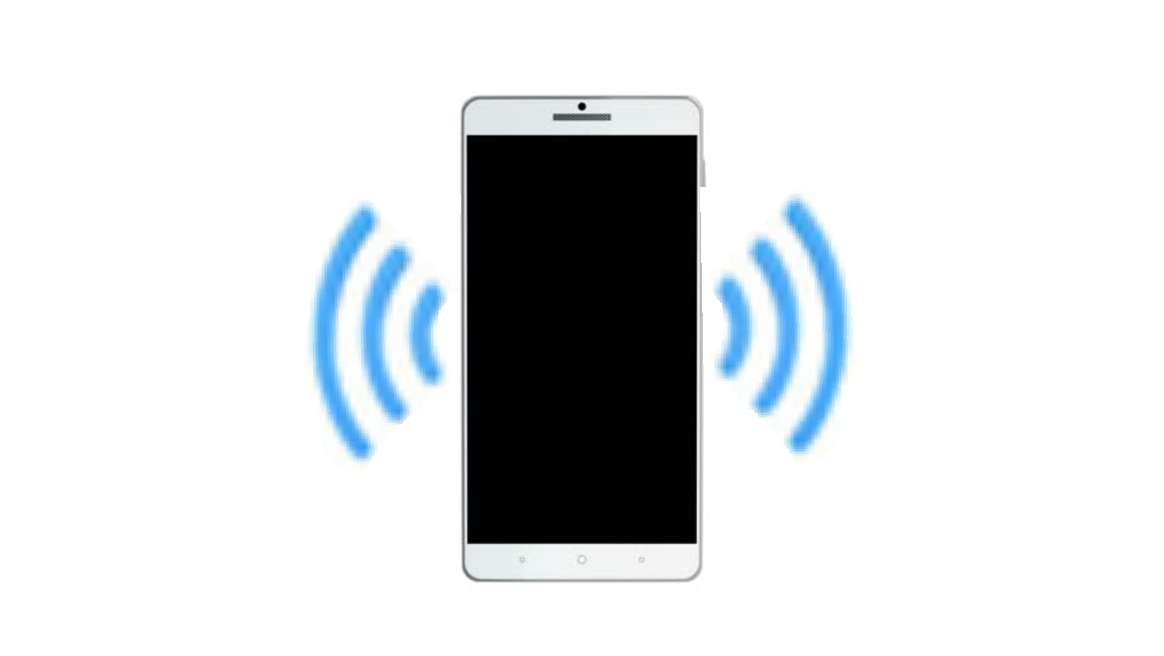
\includegraphics[width=0.09\linewidth]{img/user} \textbf{Requestor} - submits tasks to the system. Requestor submits images for text recognition
  \item[] 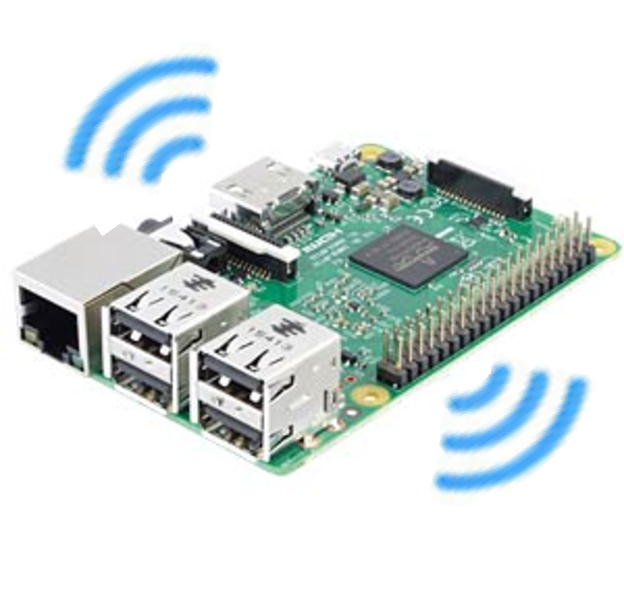
\includegraphics[width=0.07\linewidth]{img/pi} \textbf{Execution Node} - executes tasks. Execution Node accepts images, performs OCR algorithm and send back recognized text. 
  \item[] 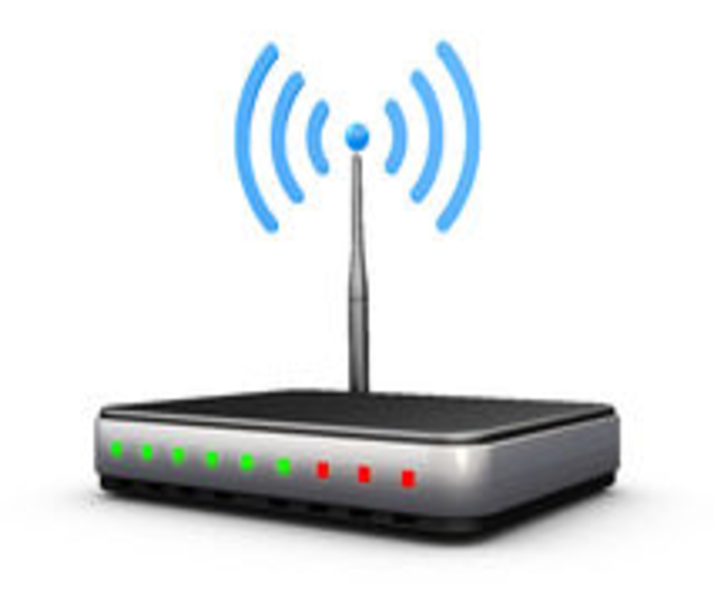
\includegraphics[width=0.07\linewidth]{img/ap} \textbf{Access Point} - performs load balancinf. Access Point implements a simple Round-Robin forwarding strategy to distribute tasks between workers. 
 \end{itemize}

\end{block}



%----------------------------------------------------------------------------------------
%	INTRODUCTION
%----------------------------------------------------------------------------------------

\begin{block}{Design Goals}

  \begin{itemize}
    \item Authenticate consumers
    \item Large parameter submission (submit a picture)
    \item In-network load balancing between multiple workers
    \item Handle PIT expiry problem when generating content
    \item Result Caching
    \item Function Migration
    
  \end{itemize}
 
\end{block}

%----------------------------------------------------------------------------------------

\end{column} % End of the first column

\begin{column}{\sepwid}\end{column} % Empty spacer column

\begin{column}{\twocolwid} % Begin a column which is two columns wide (column 2)

\begin{figure}
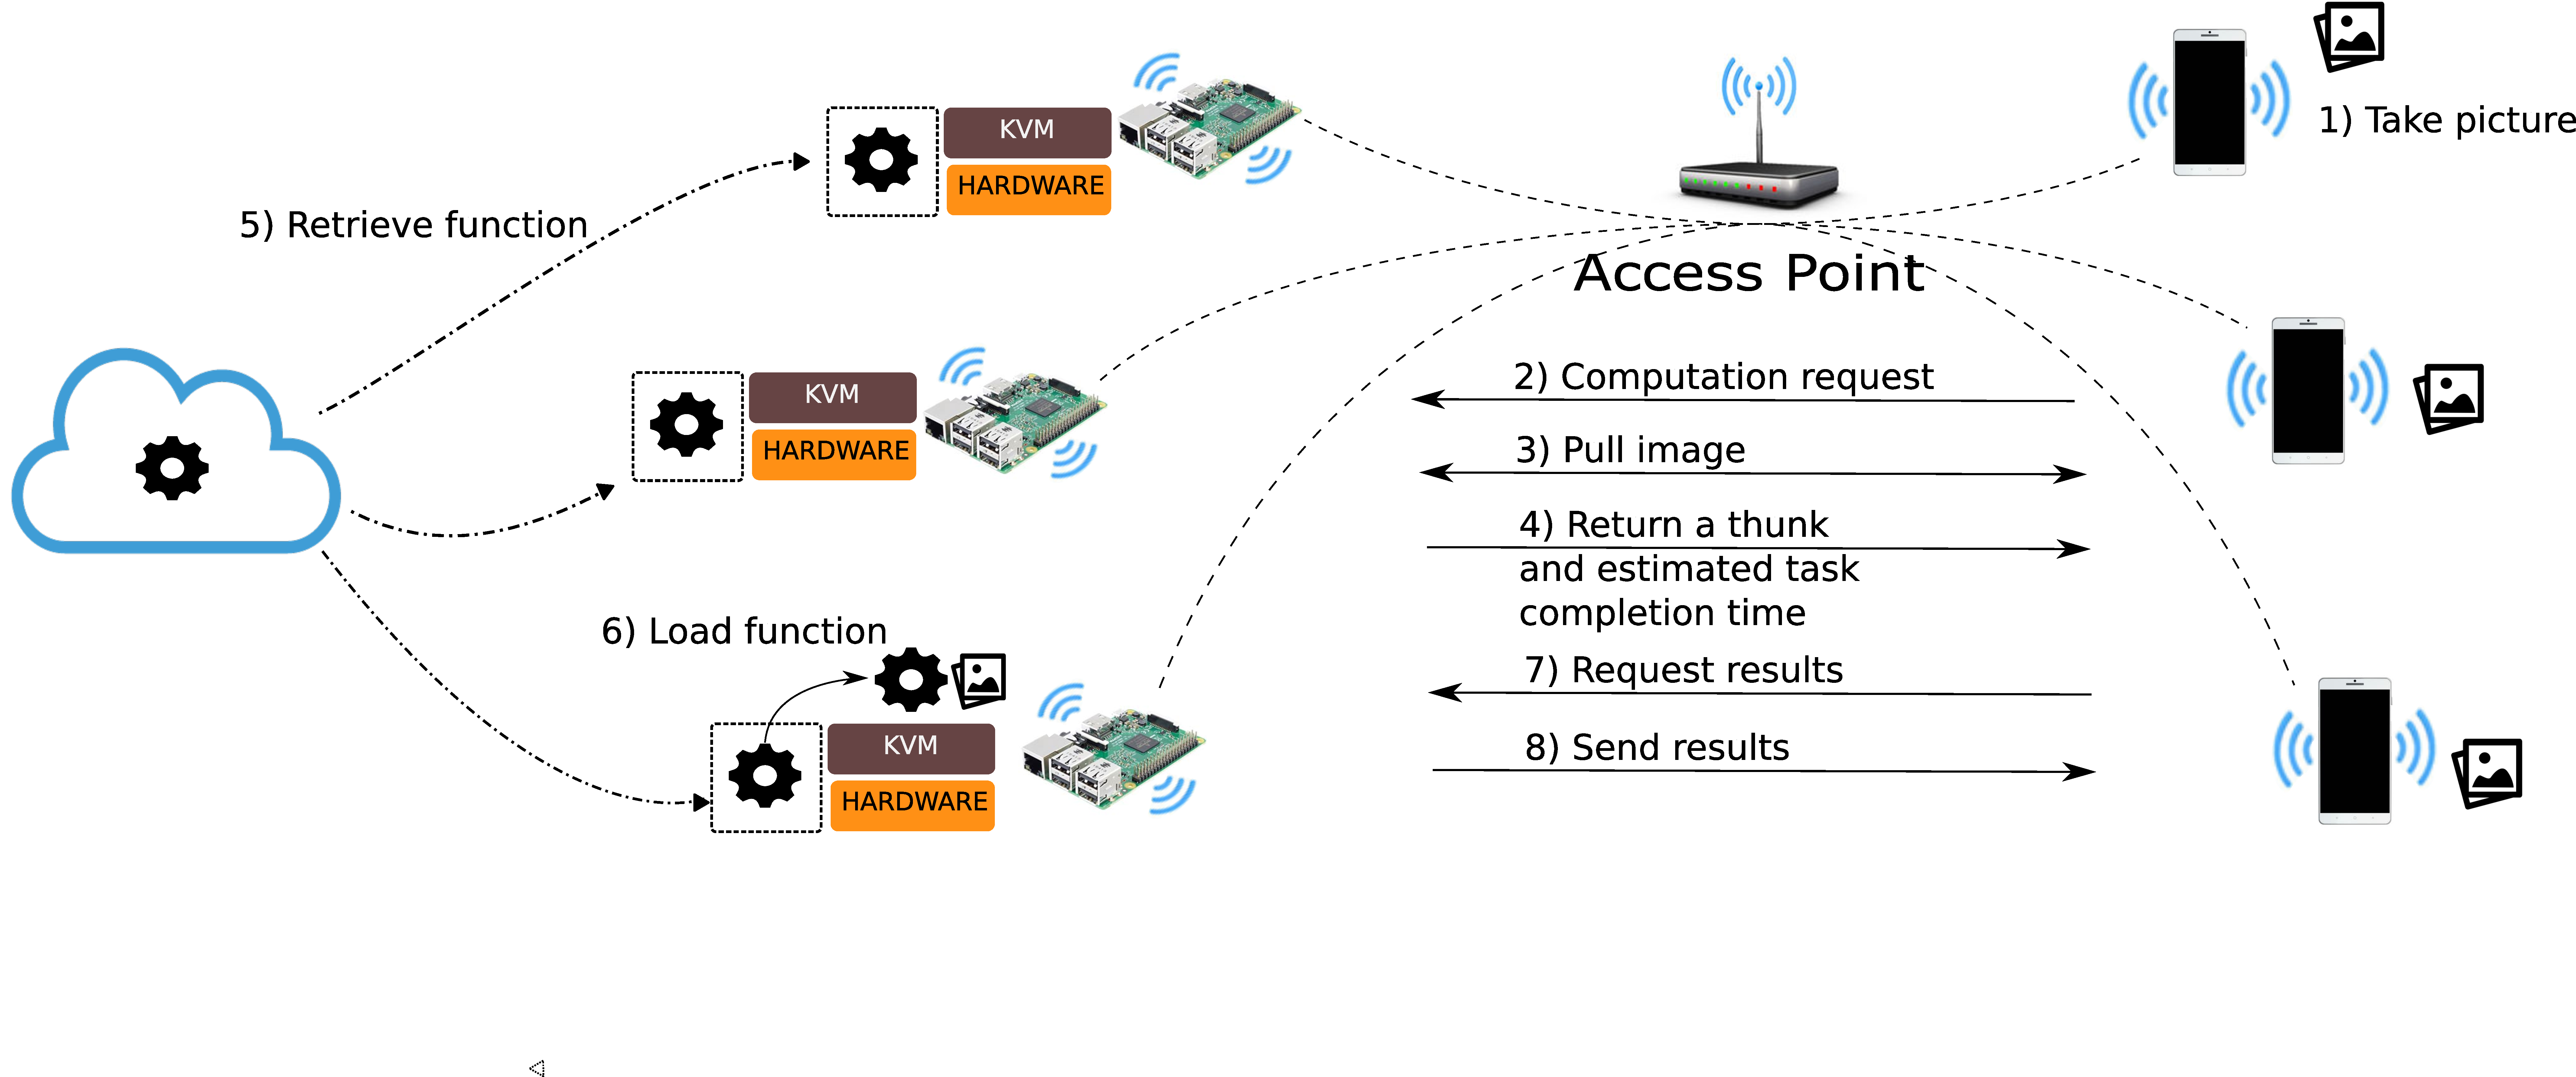
\includegraphics[width=1\linewidth]{img/scenario}
\end{figure}

%\noindent\rule{55cm}{0.4pt}

\vspace{50pt}

\begin{columns}
\begin{column}{\onecolwid}
\begin{block}{4-way Handshake}
\begin{figure}
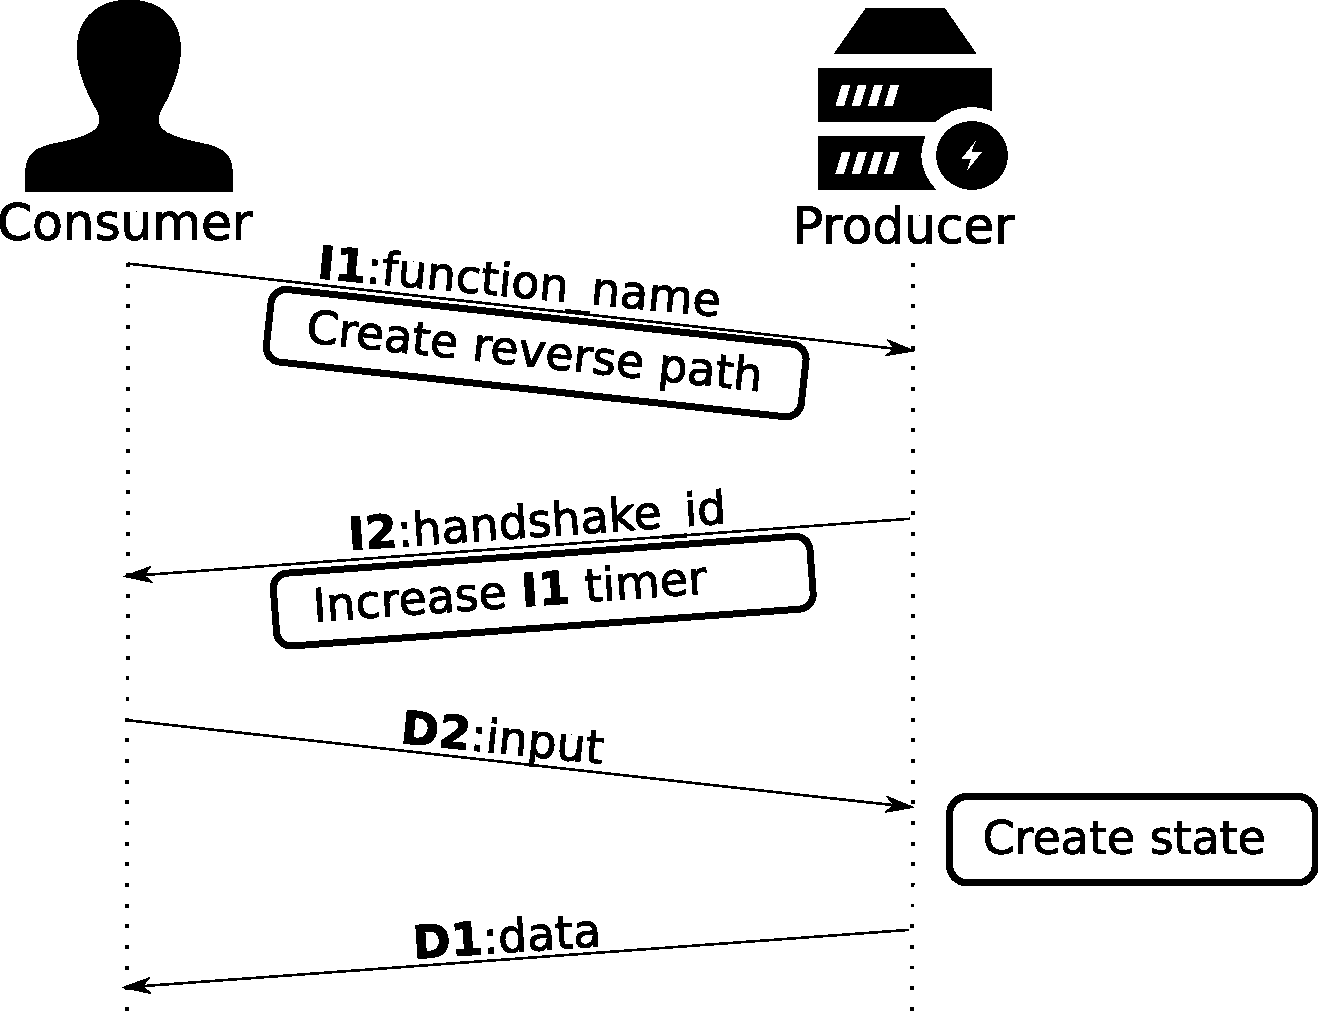
\includegraphics[width=1\linewidth]{img/handshake}
\end{figure}


\end{block}

\end{column}

\begin{column}{\onecolwid}
\begin{block}{Thunks}
\begin{figure}
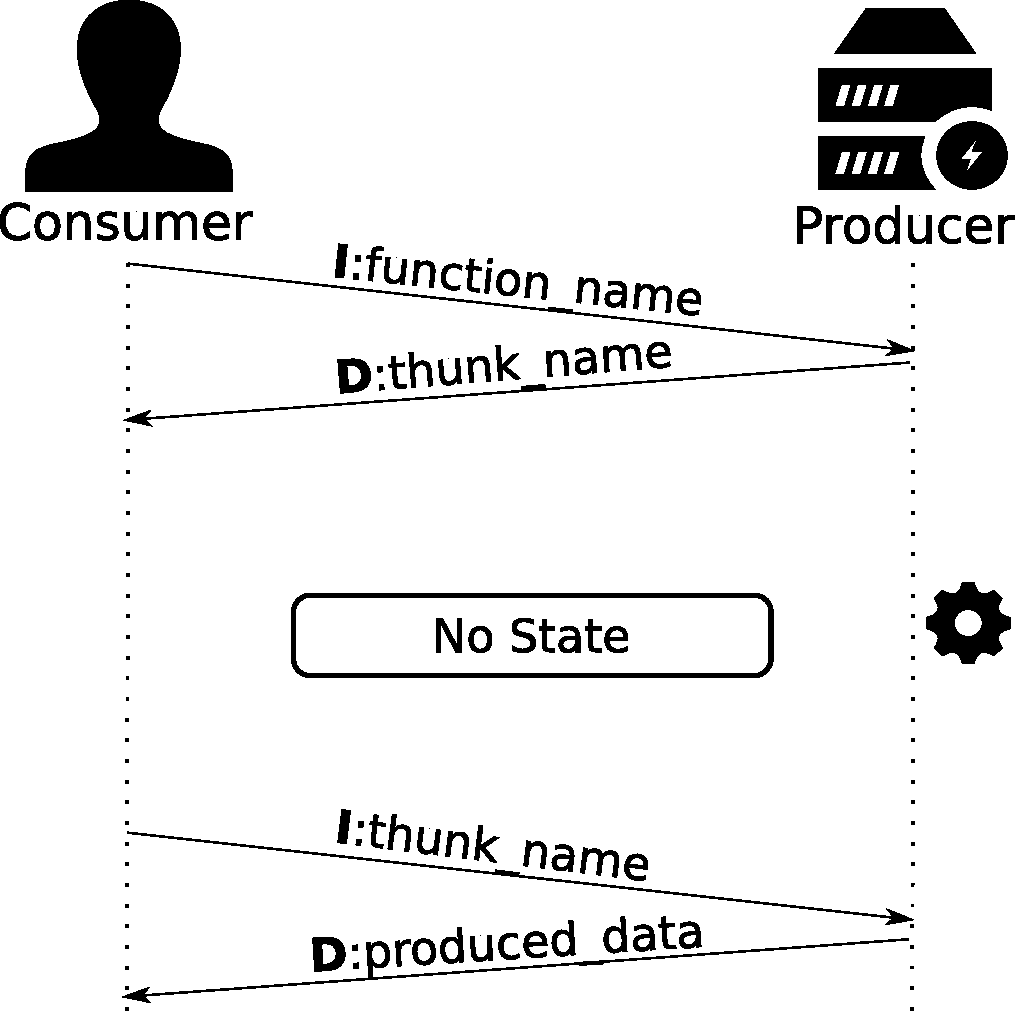
\includegraphics[width=0.8\linewidth]{img/thunks}
\end{figure}
\end{block}
\end{column}

\end{columns}



\end{column} % End of the second column

\begin{column}{\sepwid}\end{column} % Empty spacer column

\begin{column}{\onecolwid} % The third column

%----------------------------------------------------------------------------------------
%	CONCLUSION
%----------------------------------------------------------------------------------------

\begin{block}{Test it yourself}
\begin{itemize}
 \item Our application is available on Google PlayStore for Android phones.
 \item \url{https://play.google.com/store/apps/details?id=uk.ac.ucl.ndnocr}
\end{itemize}

\begin{figure}

\includegraphics[width=0.5\linewidth]{img/qr}
\end{figure}
\end{block}



%----------------------------------------------------------------------------------------
%	RESULTS
%----------------------------------------------------------------------------------------

\setbeamercolor{block alerted title}{fg=black,bg=norange} % Change the alert block title colors
\setbeamercolor{block alerted body}{fg=black,bg=white} % Change the alert block body colors

\begin{alertblock}{Results\&Future Work}
\textbf{Results}
\begin{itemize}
\item An Android application available on PlayStore.
\item No limits on the size of submitted images.
\item In-network load balncing using a simple forwarding strategy. 
\end{itemize}
\textbf{Future Work}
\begin{itemize}
\item Extend the system to use phones as workers.
\item Fully decentralized p2p network.
\item More advanced forwarding strategies for traffic shaping. 
\end{itemize}

\end{alertblock}

%----------------------------------------------------------------------------------------
%	CONCLUSION
%----------------------------------------------------------------------------------------

\begin{block}{Current Limitations}
\begin{itemize}
 \item Required accurate estimation of task completion time for optimal performance.
 \item Overestimation increases the delay.
 \item Underestimation increases the overhead.
\end{itemize}

\end{block}

%----------------------------------------------------------------------------------------

\end{column} % End of the third column

\end{columns} % End of all the columns in the poster

\end{frame} % End of the enclosing frame

\end{document}
